\chapter{Role of Tropospheric Jet Changes in the Interannual Variability and Decadal Trend of Asian Monsoon Rainfall}

\section{to-do}
1) May have to check how much Wang2013 beat you to the punch; Similarly, will have to take a long look at Ping Zhao's 2010 paper that provides an alternative coherent summary of SFND rainfall changes. 2) check rainfall changes between 1979-1993 and 1994-2007? 3) TRACK DOWN CITATION TO WANG H./WANG B./HUANG/DING/LEE paper on observed decadal change of the CGT in mid-70s; 4) Check Wang Hai email - useful information, either for Ch3 or 4?; 5) Inez had good way of summarizing Meiyu changes: 1) timing 2) frequency 3) intensity; 5) DING/WANG/WALLACE/BRANSTATOR PAPER should also be tracked down.

\section{Abstract}
We have previously investigated the leading mode of July-August Asian monsoon variability (All-Asia EOF1), distinguished by a coupling between the Himalayan Foothills and Yangtze River Valley. Here we find a robust, global shift in jet trajectory associated with positive and negative composites of All-Asia EOF1, referred to in previous work as the Circumglobal Teleconnection. Furthermore, looking specifically at East China, major late-\nth{20}-century changes in the latitude of frontal rainfall (the ``South Flood-North Drought'') coincide with anomalies in East Asian jet latitude. The East Asian tropospheric jet can influence the interannual variability of the Asian summer monsoon and vice-versa. Though the mid-latitudes force East Asian monsoon weather chaotically (the ``Silk Road'' pattern), we propose that we can improve projection of the \nth{21}-century Asian monsoon under global warming by understanding the future of the jet, for which projections are more robust. We suggest a preliminary answer to the question of what will happen to the South Flood-North Drought pattern of rainfall change in China, as well as future changes in All-Asia EOF1.

\section{Introduction}

%%KEY INTRO PARAGRAPHS?
% 1) The monsoons are the key mechanism that delivers rainfall to the tropics and subtropics. Countless studies attempt to explain their variability in terms of external forcing, including any number of oscillations...

	The global monsoon dictates a substantial fraction of the world's hydrologic budget. Typically, rainfall is delivered to monsoonal regions in abundance within a narrow seasonal window. In Asia, the timing, duration and severity of monsoon rainfall determines whether agriculture in the region will be fruitful for the year and the possibly crippling damages from floods. As a result, countless efforts have been made to prognosticate its totals and associate them to exterior modes of variability, such as ENSO, ... and ... . Some success has been made, but proper projections are likely impossible due to chaos, especially in the mid-latitudes where forecasting cannot surpass weather forecasting range by much \citep{Teng2013}.
	
% 2) Particularly key: Existing predictions of Asian monsoon climate changes are weak and potentially unfounded!
	This lack of predictability is especially problematic because even small changes in the mean state of the monsoon may impact the lives of over 4 billion people. Unfortunately, the highly heterogeneous terrain of the South and East Asian monsoons produce computational challenges that few models can resolve adequately. The IPCC5 suite of models provides no consensus on changes in the East Asian monsoon. Even this limited conformity between individual models should be viewed with skepticism. They are designed with many different types of performance objectives in mind, and may not perform well over the Asian monsoon region. Furthermore, aquaplanet versions of these models produce completely different patterns of response in future under even elementary perturbations due to the inability of models to adequately parametrize moist convection and cloud formation \citep{Stevens2013}. We suggest that the way forward lies in our knowledge of the dynamics particular to the Asian monsoon, and key components whose changes we can project.

% 3) In this chapter we investigate the role of the tropospheric jet as a potential intermediary that translates global forcing into local impacts. As the edge of the monsoon circulation, responds to changes in monsoon, but also clearly influenced by extra-tropical storminess. The jet is probably uniquely responsible in the climatology of the East Asian monsoon and its variations due to the unusual configuration of the subtropical monsoon. 
	In this work, we focus on the role of the tropospheric jet as an intermediary between global warming and regional response. At a theoretical level, the tropospheric jets marks the poleward boundaries of the Hadley Cells, and shift equatorward in summer and poleward in winter forced by insolation \citep{Bordoni2008}. A growing body of regional literature also emphasizes the importance of the shifting in Hadley Cell in regulating the inter-hemispheric energy differential. Thus, the tropospheric jet is already known to be shifting in response to forcing from global warming.

% 4) locally, the jet may take on particular importance to the South Asian and East Asian monsoon
	In East Asian summer, the jet plays an important role both in shaping the climatological distribution of rainfall and in transporting storms. The passage of the tropospheric jet north of the Tibetan Plateau summer is a precondition for the onset of the South Asian monsoon \citep{Yin1949,Yeh1959,Hahn1975}. In East Asia, a positive feedback with the Tibetan Plateau forces high-amplitude standing waves in the jet that in turn create favorable conditions for convection over China \citep{Yang2002,Molnar2010,Chen2015}. Global climate anomalies are thereby translated into unusual local weather\citep{Nigam1989,Broccoli1992,Park1997}. The jet also serves as a waveguide for storms propagating from the Eurasian interior via the ``Silk Road'' teleconnection \citep{Hoskins1993,Ambrizzi1997,Kosaka2012}. The unusually strong meridional temperature gradients in East Asia, which exist because of the presence of the Tibetan Plateau, allow for storms to propagate across much longer distances than other regions with weaker temperature gradients \citep{Branstator2002}. It is also well-known from past research that shifts in the jet's latitude and strength change patterns of storminess and rainfall in East Asia \citep{Liang1998,Branstator2002,Kwon2007,Du2009,Li2014}.  Given the interconnections between jet position and climate anomalies in Asia, if global warming has forced a jet shift, this could force changes in the mean or variability of the Asian monsoon.
	
% (may have to distinguish between subtropical jet and POLAR jet - see range of papers that discuss these two separately.
	 
	 %5) The jet should register changes in monsoon variability between years, and may also INFLUENCE its variability. We pursue this argument to its fullest extent and propose hypotheses for the future of the Asian monsoon. There may be also be local changes in the monsoons that influence the jet. 
	Given the observed interaction between the East Asian jet and Asian monsoon climatology, we expect that anomalies in each time series are also interrelated. We seek to prove two objectives: 1) That the leading mode of July-August rainfall variability, hereafter All-Asia EOF1 \citep{Day2015} also corresponds to shifts in the tropospheric jet; 2) That the South Flood-North Drought also corresponded to \nth{20}-century changes in the East Asian tropospheric jet. By associating jet changes with the leading mode and decadal trend of Asian monsoon rainfall, we may improve skill in the prediction of \nth{21}-century changes in Asian rainfall from anticipating the future of the tropospheric jet. To date even simplified models have struggled to produce consistent depictions of future changes in world climate and rainfall. By synthesizing existing literature on the future of the jet with our findings, we suggest the potential future in the variability of the East and South Asian monsoons.
	  
	%IDEA: the jet serves as a two-way intermediary between regional and global variability.
	-3 independent issues: timing, intensity and northward extent. timing being both beginning and the end, when the jet goes away. SST changes could change intensity, 
	
\section{Methods}

\subsection{Rainband Detection Algorithm (RDA) Catalog of Rainbands}

	We rely on a previously developed catalog of rainbands described and tested at length in Chapter 3.

\subsection{Jet Count Density} 

	\citet{Schiemann2009} constructed a data set of jet `counts' in the Tibetan Plateau region (46$^{\circ}$ E-130$^{\circ}$ E, 17$^{\circ}$ N-58$^{\circ}$ N) from ERA-40 reanalysis for 1958-2001, where a count is defined as any local maximum in zonal wind with westerly magnitude greater than $30$ m s$^{-1}$; further details can be found in section 2 of \citet{Schiemann2009}. We show daily mean jet latitude averaged across $90-130^\circ$E in Figure ~\ref{fig:jet_seasonal}a and monthly anomalies in Figure ~\ref{fig:jet_seasonal}b. Results are not sensitive to the choice of longitude range. Figure ~\ref{fig:climo} presents contours of jet frequency estimated by a kernel density method, which estimates a probability distribution from a set of discrete data observations.
	
	Therefore, we compare our rainband database to a database of jet counts from 1958 to 2001 from \citet{Schiemann2009} in search of coupled change. 
	
\section{All-Asia EOF1: Associated Jet Changes}

	We build composites of the most positive and negative years of All-Asia EOF1, and compare their upper-tropospheric wind anomalies to. The pattern of meridional wind changes corresponding to the inter-composite difference. This pattern strongly resembles the spatial arrangement of the Circumglobal Teleconnection studied in \citet{Ding2005a}, which is a zonal wavenumber 5 Rossby wavetrain that spans the entire globe. \citet{Branstator2002} found that, in regions of strong meridional temperature gradient such as East Asia, a pattern with zonal wavenumber 5 can extend around the globe, with the tropospheric jet serving as a waveguide favoring the zonal propagation of storms. Their Figure 1c in that text is very similar to our result. \citet{Ding2007} further investigated the daily evolution of a Eurasian wavetrain pattern bearing strong resemblance to the CGT. In their estimation, the original forcing lies in the region of the North Atlantic jet exit, a region of very high variability in geopotential height. The downstream propagation of signals from this region then controls active and break spells in the Indian monsoon, equivalent to forcing India EOF1 positively or negatively. The diabatic heating from the Indian monsoon then further strengthens the Central Asian high, which in turn can trigger a Siberian high that brings anomalous rainfall to North China. We suggest that our hypothesis of moisture transport linking the Himalayan Foothills to the Yangtze River Valley \citep{Day2015} is not incompatible with their theory - our mechanism and theirs could be mutually reinforcing.

\section{The ``South Flood-North Drought:'' Associated Jet Changes}

\section{Climatology of the East Asian Jet}

	The East Asian jet is closely associated with the five rainfall stages of East Asian monsoon rainfall described in Chapter 3. Beginning in May, the East Asian jet moves from its winter position on the southern flank of the Tibetan Plateau to a summer latitude well north of the plateau.  A full monthly jet climatology is visible in \citet{Schiemann2009}; During this transition, the jet occupies intermediate configurations that correspond to different stages of China rainfall (Figure ~\ref{fig:climo}). Peak rainfall rates in China from May to mid-July corresponds to the months when the climatological latitude of the jet impinges on the Tibetan Plateau, because the interaction of the tropospheric jet and Tibetan Plateau strengthens convergence and rainfall downstream over China and the western Pacific Ocean \citep{Molnar2010,Sampe2010,Chen2014}. From May to September,  the climatological latitude of rainfall, rainbands and jet density are all closely coupled, with peak jet density occurring 5 to 10 degrees north of the latitude of peak rainfall. This agrees with the prediction that, in a region of strong frontal conditions as observed in East Asia, the co-occurrence of a strong upper-tropospheric jet and a coupled equatorward region of ascent and strong rainfall \citep{Holton2004}. 
	
	The initiation of the Pre-Meiyu corresponds roughly to the beginning of the jet's northward passage. During Meiyu season, the preferred latitude of the jet continues to shift northward. The period of frequent double rainband occurrence during the Post-Meiyu corresponds to the jet's maximal northward extent. Finally, the jet returns southward during the Fall Rains in October and November, which produces only a weak rainfall response.
	
	In addition, Figures ~\ref{fig:climo}a-e show mean rainfall, jet frequency and rainband position during each stage, as well as their zonal average (sidebars). From the Pre-Meiyu to Post-Meiyu, each northward jump in peak rainband frequency corresponds to a similar shift in jet count density, with a southward offset of about 5 degrees.
	
\subsection{Jet Changes, 1980-2001 Versus 1958-1979}

	In Figure ~\ref{fig:jet_seasonal}a, we show the zonal average over $90-130^\circ$E) of mean jet latitude, averaged over the years 1958-1979 (blue solid line) and 1980-2001 (dashed red line) with 95\% confidence intervals overlain. Both significant changes in rainband statistics described in the previous section correspond to southward shifts in mean jet latitude. During the Pre-Meiyu (May), the tropospheric jet is shifted southward by almost 2$^{\circ}$ in 1980-2001 relative to 1958-1979, when its mean latitude was $\approx 41^{\circ}$N. We estimate the significance of this change using a two-tailed Kolmogorov-Smirnov (K-S) test. Since the K-S test requires that all samples are independent, we first remove temporal autocorrelation due to synoptic variability by assimilating daily mean jet latitude into 4 day blocks. A subsequent K-S test finds that the shift is significant with $p=0.003998$. During the Post-Meiyu (days 201-273), when a southward shift in rainband latitude is found in 1980-2001 relative to 1958-1979, the mean latitude of the jet is also consistently displaced southward. We assimilate daily mean jet latitude into 7-day blocks before performing a K-S test, and find a $p$-value of this shift of $p=0.05667$.
	
\section{Hypothesis}

	The Meiyu front and tropospheric jet covary in latitude from May to September in the climatological mean, and parallel changes are found in rainband attributes and mean jet latitude between 1951-1979 and 1980-2007. Therefore, the South Flood-North Drought appears to reflect an alteration in jet dynamics. We propose that both the Pre-Meiyu decline in rainband frequency and the Post-Meiyu southward shift of rainband latitude result from a single phenomenon: an overall southward displacement of the jet's summer progression over East Asia. In climatology, the Pre-Meiyu corresponds to both a surge in rainfall and the beginning of the jet's northward transit, when its preferred latitude begins to impinge on the Tibetan Plateau. We propose that the observed southward shift in the jet during May has delayed the date when the jet first impinges on the Tibetan Plateau, resulting in a delay in Pre-Meiyu onset and prolonged Spring Rain conditions. This is manifested as weaker rainfall and decreased rainband frequency in central China in May. Subsequently, we argue that the reduced northward extent of the jet during the Post-Meiyu has shifted rainfall and mean rainband latitude southward. Finally, we suggest that the southward displacement of the summer jet cycle results in a decrease in northern China annual rainfall and an increase in central China annual rainfall, producing a South Flood-North Drought response. Thus, our hypothesis can explain the major observed changes in rainfall and rainband statistics during the Pre- and Post-Meiyu as well as cumulative yearly change.
	
	To test our hypothesis, we investigate the relation of interannual anomalies in jet latitude and rainband properties. Figure ~\ref{fig:jet_seasonal}b shows a scatter plot of rainband \textit{frequency} anomalies versus jet latitude anomalies in May (days 121-150). Most years with a decrease in rainband frequency feature a southward jet shift, and vice-versa, and such years occur mostly during 1980-2007. A similar relation is found between monthly anomalies in rainband \textit{latitude} and jet latitude during July-August (days 201-260, Figure ~\ref{fig:jet_seasonal}c). In the latter figure, we exclude rainbands south of 28$^{\circ}$ N from calculated anomalies, since such rainbands reflect South China Sea storms, rather than jet influence \citep{Day2015}. Together, Figures ~\ref{fig:jet_seasonal}b and ~\ref{fig:jet_seasonal}c suggest that interannual changes in jet latitude affect Pre-Meiyu rainband frequency and Post-Meiyu rainband latitude.
	
	 %%should probably move away from previous conclusion that jet shifts caused SFND, because causality difficult to distinguish - but, still reasonable to suggest that we can get more predictive skill on the monsoon by understanding future jet changes.
	 	 
	We propose that the delayed passage of the jet to the north of the Tibetan Plateau has shortened the Pre-Meiyu season, decreasing May rainfall in central China, and restricted the northward advance of precipitation, consequently reducing Post-Meiyu rainfall in northern China. This interpretation is a modern analog of the ``Jet Transition Hypothesis'' described in \citet{Chiang2015}, wherein East Asian rainfall changes on paleoclimate timescales are ascribed to modulation in the seasonal cycle of the tropospheric jet. 	
 		 
\section{Potential for Constrained Projection}

\subsection{Key Argument}
	%% KEY ARGUMENT
	Causality is difficult to distinguish. The different elements of the Asian monsoon must shift in physically consistent manner, but this does not reveal the initial trigger. The jet changes in the SFND may indeed be simply a local response to patterns of diabatic heating. Nonetheless, we suggest that the historical association between them means that \textit{we can constrain the sample space of future changes in the Asian monsoon by predicting future changes in the jet}.
	
\subsection{Historical trends in the jet}
	%historical jet changes
	Observations show that the global annual mean latitude of the tropospheric jet has shifted poleward, in tandem with tropospheric heating and lower-stratospheric cooling in the mid-latitudes, increased subtropical static stability, and the expansion of the Hadley circulation \citep{Fu2006,Archer2008,Fu2011}. Opposite trends are found in some regions and the variation by season is significant; we find that the East Asian portion of the jet has shifted equatorward, in agreement with past studies \citep{Yu2007, Archer2008}. Recent work proposes that the observed southward displacement of the jet over the Pacific Ocean was caused by \nth{20}-century changes in tropical Pacific convection and SST \citep{Park2014a}. Thus, the global poleward trend in jet latitude and the East Asian equatorward shift are compatible observations that reflect the heterogeneous spatial distribution of \nth{20}-century warming.

\subsection{Future changes}
\subsubsection{CMIP5 consensus}
	%IPCC5 consensus paragraph - kinda boring, so keep short. should list the caveats of CMIP5 talks
	\citet{Lee2014} analyzed \nth{21}-century changes in a suite of CMIP5 models and concluded that the robust stabilization of the atmosphere in almost all models would tend to decrease the variability associated with the CGT. However, these models may suffer from the fundamental issue of being targeted to hit the mean, and therefore not exploring a suitable range of unlikely scenarios. The state of future projections for the Asian monsoon is highly uncertain. The ability of many models out of IPCC to simulate basic features of the South and East Asian monsoon remains in question.

\subsubsection{Idealized studies}
	%Consensus about the future jet from modeling work'
	The poleward expansion of the Hadley Cell is projected to continue under \nth{21}-century warming \citep{Frierson2007,Lu2007,Kang2012}, but a recent study predicts that anomalous \nth{21}-century heating of the eastern Pacific Ocean will drive the Pacific jet further equatorward \citep{Park2014}.
	
	

	%IMPLICATIONS for monsoon	
		 
\section{Conclusion}

	We have shown that a significant amount of the annual and decadal variability in Meiyu front activity is accompanied by changes in the westerly jet. Two major changes in the progression of the East Asian summer monsoon were previously reported: 1) A decrease in frequency during the Pre-Meiyu season (days 121-160, May 1-June 9; $p=.0019$); and 2) A southward shift in rainband latitude during the Post-Meiyu season (days 201-273, July 20-Sep 30; $p=.0003$). The latter change is responsible for the South Flood-North Drought trend in total yearly rainfall. In addition, both time periods display a southward anomaly in mean jet latitude during 1980-2007 relative to 1951-1979. We argue that both Pre-Meiyu and Post-Meiyu changes in rainfall and rainband statistics are caused by a southward shift of the summer progression of the East Asian tropospheric jet. In particular, we propose that the delayed passage of the jet to the north of the Tibetan Plateau has shortened the Pre-Meiyu season, decreasing May rainfall in central China, and restricted the northward advance of precipitation, consequently reducing Post-Meiyu rainfall in northern China. This interpretation is a modern analog of the ``Jet Transition Hypothesis'' described in \citet{Chiang2015}, wherein East Asian rainfall changes on paleoclimate timescales are ascribed to modulation in the seasonal cycle of the tropospheric jet. 	
 
	Many components of our results have been presented in previous work. \citet{Xuan2011} find a southward shift in the jet and increased Yangtze Valley rainfall in July. \citet{Yu2004} and \citet{Yu2007} found a southward shift in July-August jet latitude and suggested a link with the South Flood-North Drought. Potential mechanisms for late \nth{20}-century East Asian climate change include changes in Indian Ocean SST \citep{Qu2012}, decreased sensible heating from the Tibetan Plateau \citep{Liu2012a,Hu2015} and aerosol forcing \citep{Song2014}.
	
 By linking the South Flood-North Drought to changes in the seasonal advance of the tropospheric jet, we open the possibility of projecting \nth{21}-century East Asian rainfall change by improving our understanding of the effect of further global warming on the regional and global behavior of the tropospheric jet.
	
	%%VERY LAST PARAGRAPH - ANY INTUITION ON THE FUTURE OF THE SFND?
	
\section{Acknowledgments}

	Significant portions of the current work were produced in collaboration with Jacob Edman and John Chiang and under the guidance of Inez Fung.


%% FIGURE 4.1 Climatology of rainfall stages including rainfall, jet and most likely rainband configuration, and longitudinal averages.
\begin{figure}
\centering
\noindent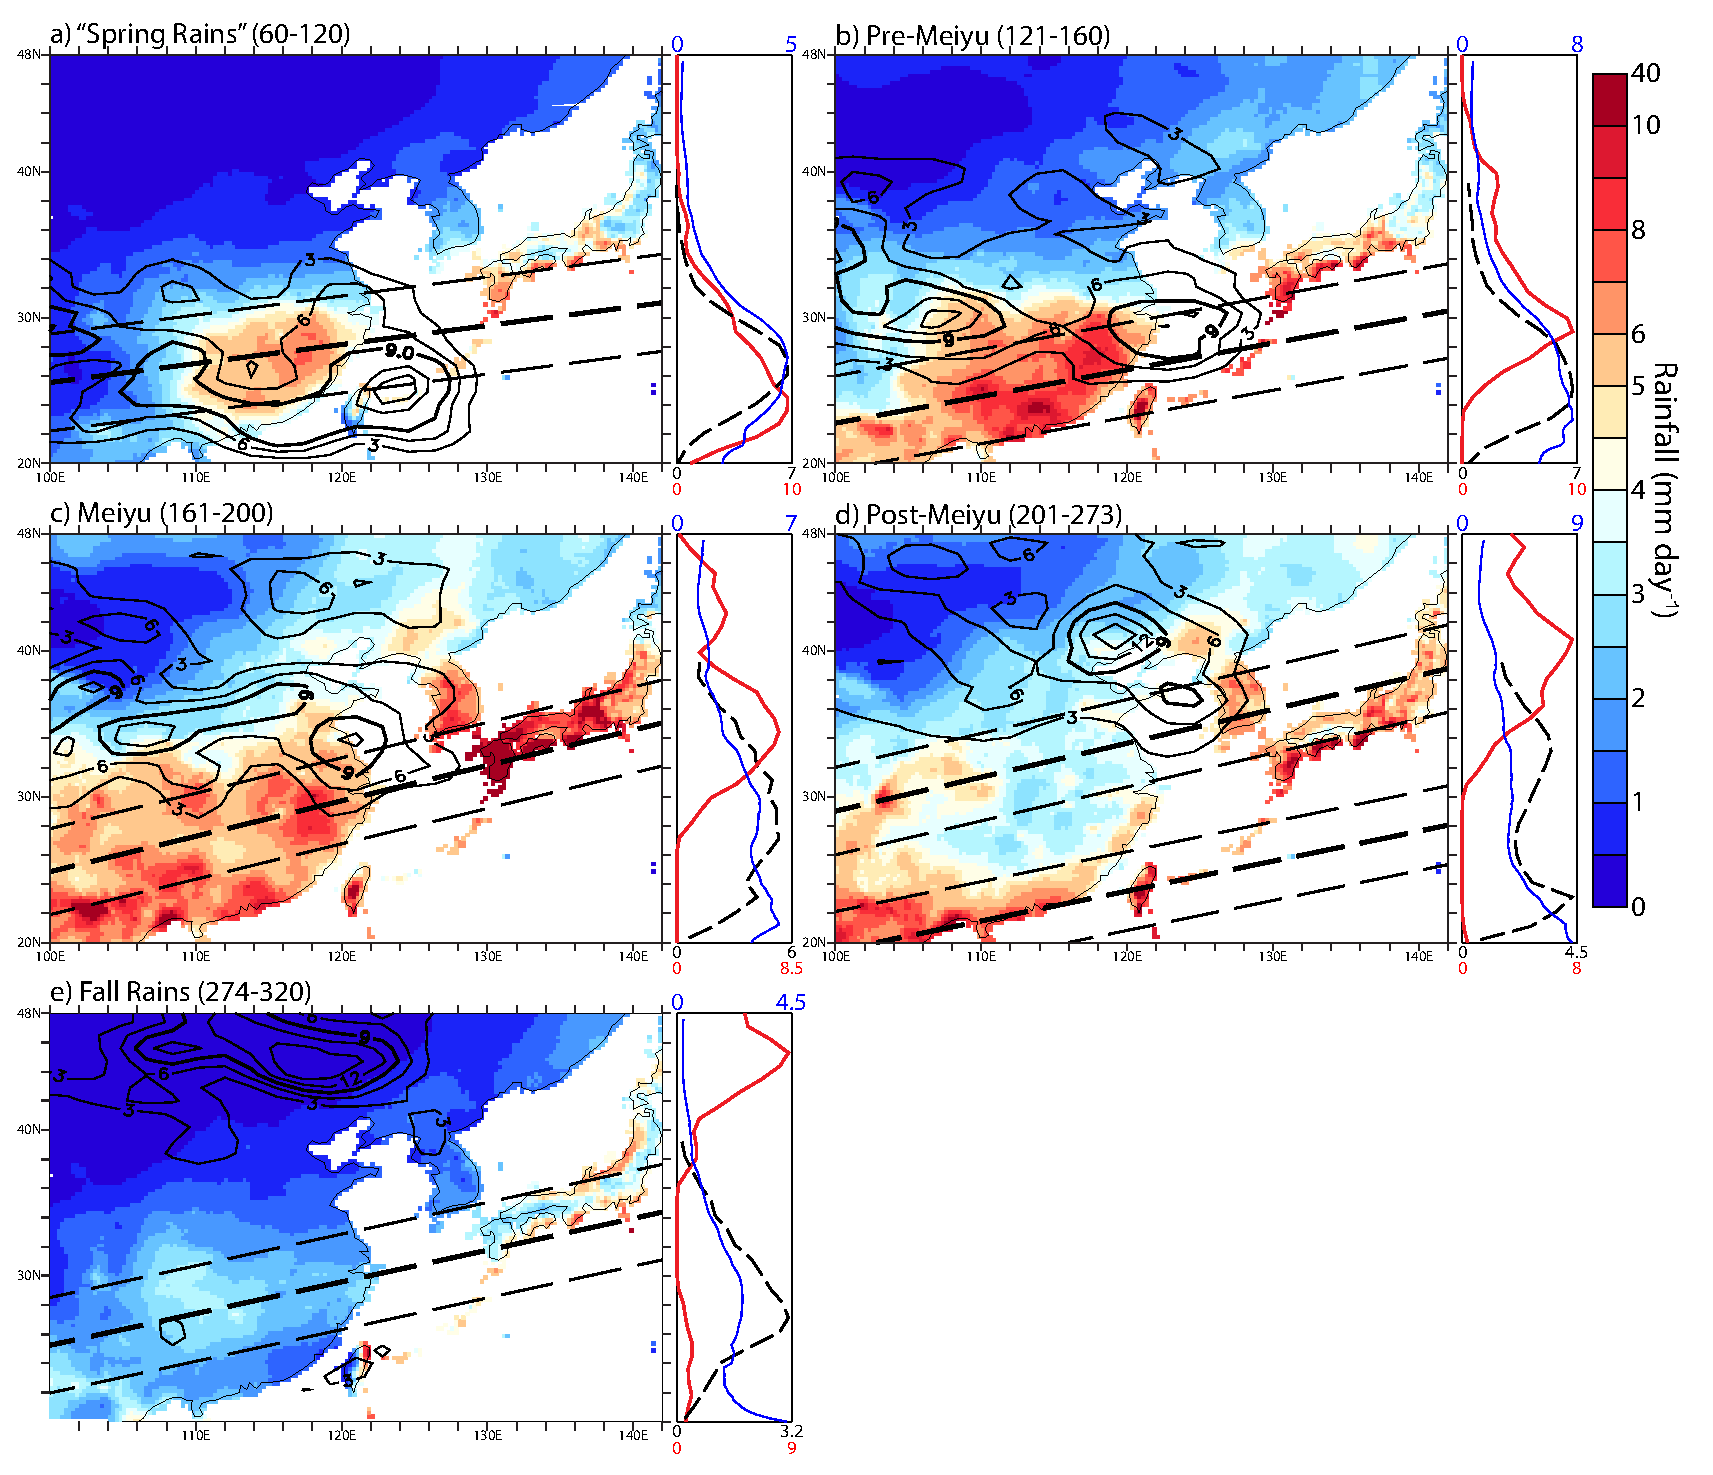
\includegraphics[width=36pc]{Figures/ch4/climo}
\caption{Climatology of East Asian rainfall stages showing rainfall (shading), jet kernel density (contours of probability density in units of $10^{-4}$) and most common rainband position during that stage. Sidebars shows, for each time period, the longitude average over 105-123$^{\circ}$E of rainfall (thin blue line, units of mm day$^{-1}$), jet kernel density (red line, units of $10^{-4}$) and rainband position (dashed black line, absolute probability in \%, 1-degree latitude smoothing). From the Pre-Meiyu to Post-Meiyu, a peak in preferred jet latitude consistently occurs 5 degrees north of a corresponding maximum in rainband frequency.}
\label{fig:climo}
\end{figure}


%% FIGURE 4.2 - 2D spatial distribution of change showing a) full year b) Pre-Meiyu and c) Post-Meiyu
\begin{figure}
\centering
\noindent\includegraphics[width=36pc]{Figures/ch4/changes_2d_jet}
\caption{a) Whole year mean rainfall change, showing the South Flood-North Drought pattern; b) Rainfall changes during the Pre-Meiyu (days 121-160) with contours of jet density change overlain; c) Same as c, but for the Post-Meiyu (days 201-273). Statistical significance at 95\%/99\% level overlain with single/double hatches. Sidebars show, for each time period, the longitude average over 105-123$^{\circ}$E of changes in rainfall (thin blue line, units of mm day$^{-1}$), jet kernel density (red line, units of $10^{-4}$) and rainband position (dashed black line, absolute probability in \%, 1-degree latitude smoothing).}
\label{fig:changes_2d}
\end{figure}

%% FIGURE 4.3 - Changes in jet mean between 1951-1979 and 1980-2007 + scatter plots of jet and rainband monthly anomalies.
\begin{figure}[htbp]
\centering
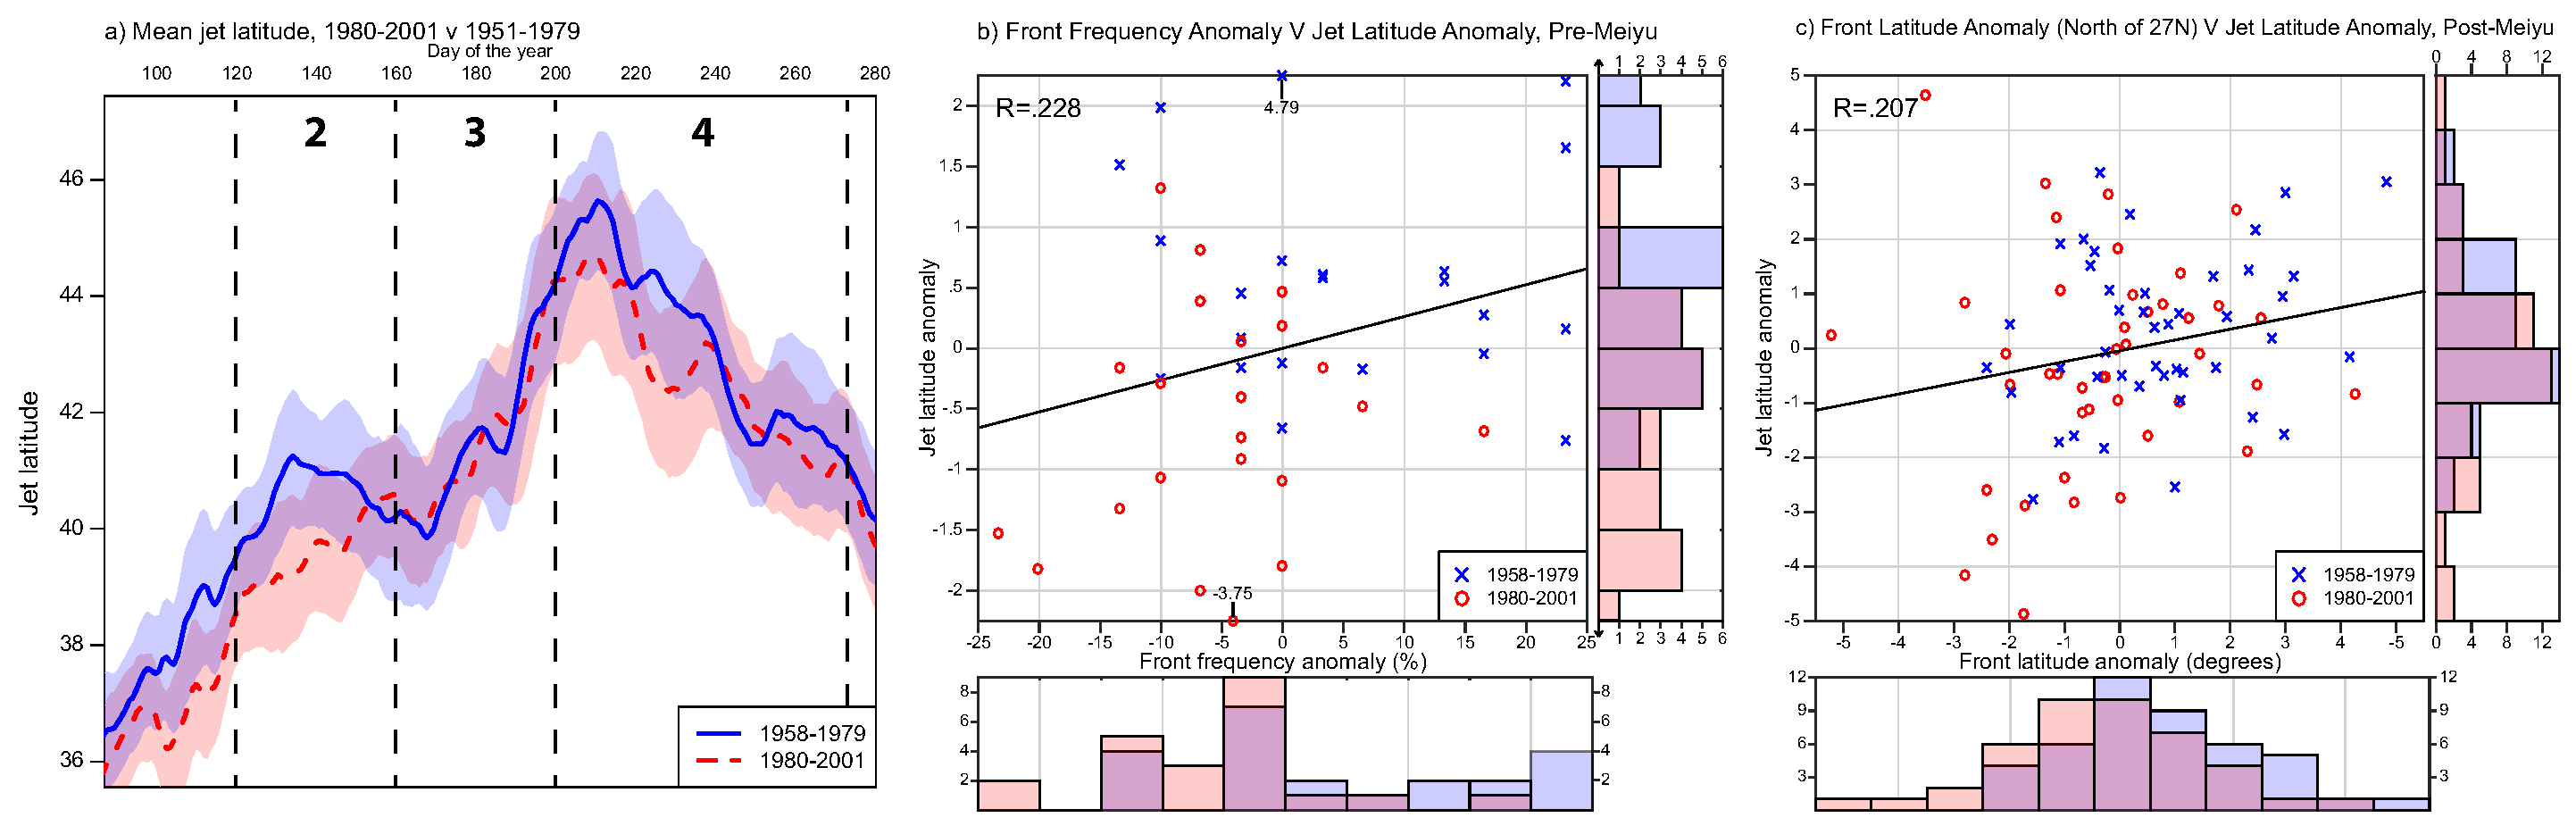
\includegraphics[width=42pc]{Figures/ch4/jet}
\caption{a) 7-day running mean latitude of the westerly jet in the region 90-130$^\circ$E for the years 1958-1979 (blue, solid) and 1980-2001 (red, dashed). Bootstrapped 95\% confidence intervals are shaded. Time periods: 2 - Pre-Meiyu; 3 - Meiyu; 4 - Post-Meiyu; b) Plot of monthly anomalies in rainband frequency versus monthly anomalies in jet latitude during days 121-150 (May) for 1958-1979 (blue X) versus 1980-2001 (red circle); c) Same as b), but showing 30-day anomalies of rainband latitudes during the Post-Meiyu (201-230 and 231-260, each set of 30 days treated as a separate point). Histograms of anomalies are also shown on the side of each figure.}
\label{fig:jet_seasonal}
\end{figure}

%% FIGURE 4.4 - Temporal autocorrelation of the jet used to demonstrate the choice of block size for averaging.
\begin{figure}[htbp]
\centering
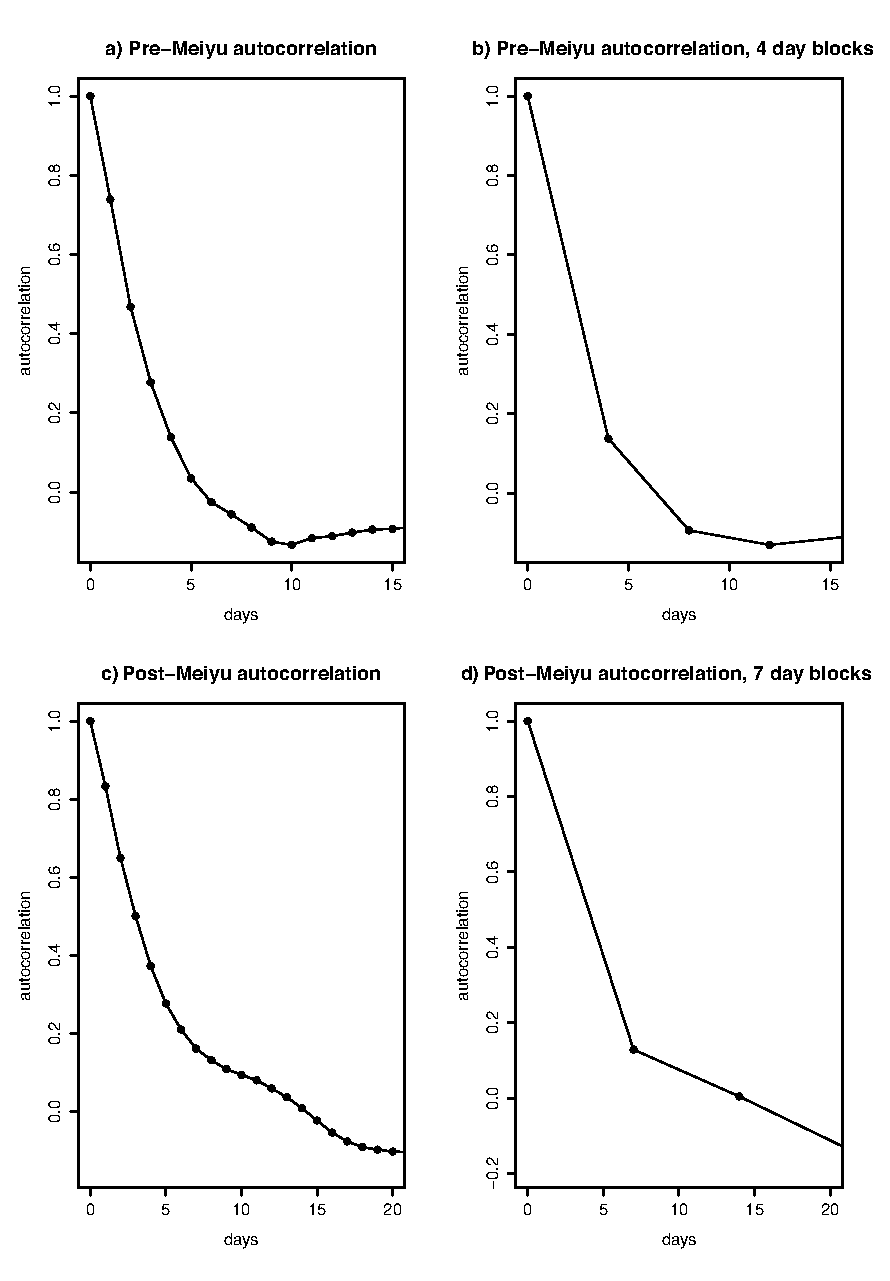
\includegraphics[width=42pc]{Figures/ch4/jet_autocorr}
\caption{The accumulation of the jet into blocks eliminates the autocorrelation from the daily mean latitude signal. During the Pre-Meiyu, mean daily jet latitude is further smoothed over 4 days (panels a and b); During the Post-Meiyu, we average over 7 days (panels c and d).}
\label{fig:jet_autocorr}
\end{figure}
